\documentclass{beamer}

\mode<presentation>
{
  \usetheme{Szeged}
  \usecolortheme{seagull}
}

%\usepackage[english]{babel}
\usepackage{float}
\usepackage{subcaption}
\usepackage{amsmath}
\usepackage{braket}
\usepackage{multirow}
\graphicspath{{./images/}}

% footnote references
\usepackage{natbib}
\usepackage{bibentry}
\bibliographystyle{plain}
\usepackage{chngcntr}
\counterwithin*{footnote}{page}
\newcommand\footcite[1]{\footnote{\bibentry{#1}}\label{\thepage:#1}}
\newcommand\secondcite[1]{\textsuperscript{\ref{\thepage:#1}}}
\setbeamerfont{footnote}{size=\tiny}

\usepackage[utf8]{inputenc}

\usepackage{times}
\usepackage[T1]{fontenc}


\title{Progress Report}
\date

\author{Daniel Pereira}


\institute[Instituto de Telecomunições] % (optional, but mostly needed)

\date

\pgfdeclareimage[height=0.5cm]{university-logo}{logo-IT-header.png}
\logo{\pgfuseimage{university-logo}}

\AtBeginSection[]{
  \begin{frame}
  \vfill
  \centering
  \begin{beamercolorbox}[sep=8pt,center,shadow=true,rounded=true]{title}
    \usebeamerfont{title}\insertsectionhead\par%
  \end{beamercolorbox}
  \vfill
  \end{frame}
}

\AtBeginSubsection[]{
  \begin{frame}
  \vfill
  \centering
  \begin{beamercolorbox}[sep=8pt,center,shadow=true,rounded=true]{title}
    \usebeamerfont{title}\insertsubsectionhead\par%
  \end{beamercolorbox}
  \vfill
  \end{frame}
}

%\AtBeginSection[]
%{
%  \begin{frame}<beamer>{Índice}
%    \tableofcontents[currentsection]
%  \end{frame}
%}



\begin{document}
\nobibliography{beamer}
\begin{frame}
  \titlepage
\end{frame}

\begin{frame}{Index}
  \tableofcontents
% You might wish to add the option [pausesections]
\end{frame}



%%%%%%%%%%%%%%%%%%%%%%%%%%%%%%%%%%%%%%%%%%%%%%%%%%%%%%%%%%%%%%%%%%%%%%%%%%
%%%%%%%%%%%%%%%%%%%%%%%%%%%%%%%%%%%%%%%%%%%%%%%%%%%%%%%%%%%%%%%%%%%%%%%%%%
%%%%%%%%%%%%%%%%%%%%%%%%%%%%% section 1 %%%%%%%%%%%%%%%%%%%%%%%%%%%%%%%%%%
%%%%%%%%%%%%%%%%%%%%%%%%%%%%%%%%%%%%%%%%%%%%%%%%%%%%%%%%%%%%%%%%%%%%%%%%%%
%%%%%%%%%%%%%%%%%%%%%%%%%%%%%%%%%%%%%%%%%%%%%%%%%%%%%%%%%%%%%%%%%%%%%%%%%%
\section{Introduction}
\begin{frame}[t]{Objectives}
\begin{itemize}
\item Study CV-QKD with 4 state discrete modulation.
\item Both simulation and experimental results where obtained.
\item Results where linked to theoretical expected values, not each other (missing detector information to compare simulation to experimental values).
\end{itemize}
\end{frame}

\begin{frame}[t]{Results in this Presentation}
\begin{itemize}
\item Simulation results:
\begin{itemize}
\item Noise characterization.
\item Secret key generation rate in function of transmission for two levels of excess noise.
\end{itemize}
\item Experimental results:
\begin{itemize}
\item Phase drift compensation.
\item Noise characterization experiment.
\item Key distribution experiment with secret key generation rate estimation.
\end{itemize}
\end{itemize}
\end{frame}

%%%%%%%%%%%%%%%%%%%%%%%%%%%%%%%%%%%%%%%%%%%%%%%%%%%%%%%%%%%%%%%%%%%%%%%%%%
%%%%%%%%%%%%%%%%%%%%%%%%%%%%%%%%%%%%%%%%%%%%%%%%%%%%%%%%%%%%%%%%%%%%%%%%%%
%%%%%%%%%%%%%%%%%%%%%%%%%%%%% section 2 %%%%%%%%%%%%%%%%%%%%%%%%%%%%%%%%%%
%%%%%%%%%%%%%%%%%%%%%%%%%%%%%%%%%%%%%%%%%%%%%%%%%%%%%%%%%%%%%%%%%%%%%%%%%%
%%%%%%%%%%%%%%%%%%%%%%%%%%%%%%%%%%%%%%%%%%%%%%%%%%%%%%%%%%%%%%%%%%%%%%%%%%
\section{Theoretical notes}
\begin{frame}[t]
\begin{align*}
K&=\beta I(A:B)-S(B:A) = \beta\log_2(1+\text{SNR})-S(AB)+S(AB|B)\\
&=\beta\log_2(1+\text{SNR}) -\sum_{k=1}^2\left[(\bar{n}_k^{AB}+1)\log_2(\bar{n}_k^{AB}+1)-\bar{n}_k^{AB}\log_2\bar{n}_k^{AB}\right]\\
&\qquad {} \qquad {}  \qquad {} \qquad {}   +(\bar{n}^{AB|B}+1)\log_2(\bar{n}^{AB|B}+1)-\bar{n}^{AB|B}\log_2\bar{n}^{AB|B}
\end{align*}
\end{frame}

\begin{frame}[t]
\begin{align*}
\gamma_\text{AB}=\left[
\begin{matrix}
(1+2\braket{n})\mathbb{I}_2 & \sqrt{\frac{T}{2}}Z\sigma_Z \\
\sqrt{\frac{T}{2}}Z\sigma_Z & (T\braket{n}+1+\frac{T}{2}\epsilon)\mathbb{I}_2 
\end{matrix}
\right]
\end{align*}
\begin{align*}
\gamma_{AB|B}=\left[(1+2\braket{n})-\frac{\frac{T}{2}Z^2}{T\braket{n}+2+\frac{T}{2}\epsilon}\right]\mathbb{I}_2
\end{align*}
\end{frame}

%%%%%%%%%%%%%%%%%%%%%%%%%%%%%%%%%%%%%%%%%%%%%%%%%%%%%%%%%%%%%%%%%%%%%%%%%%
%%%%%%%%%%%%%%%%%%%%%%%%%%%%%%%%%%%%%%%%%%%%%%%%%%%%%%%%%%%%%%%%%%%%%%%%%%
%%%%%%%%%%%%%%%%%%%%%%%%%%%%% section 3 %%%%%%%%%%%%%%%%%%%%%%%%%%%%%%%%%%
%%%%%%%%%%%%%%%%%%%%%%%%%%%%%%%%%%%%%%%%%%%%%%%%%%%%%%%%%%%%%%%%%%%%%%%%%%
%%%%%%%%%%%%%%%%%%%%%%%%%%%%%%%%%%%%%%%%%%%%%%%%%%%%%%%%%%%%%%%%%%%%%%%%%%
\section{Simulation}
\begin{frame}[t]{Block diagram}
\begin{center}
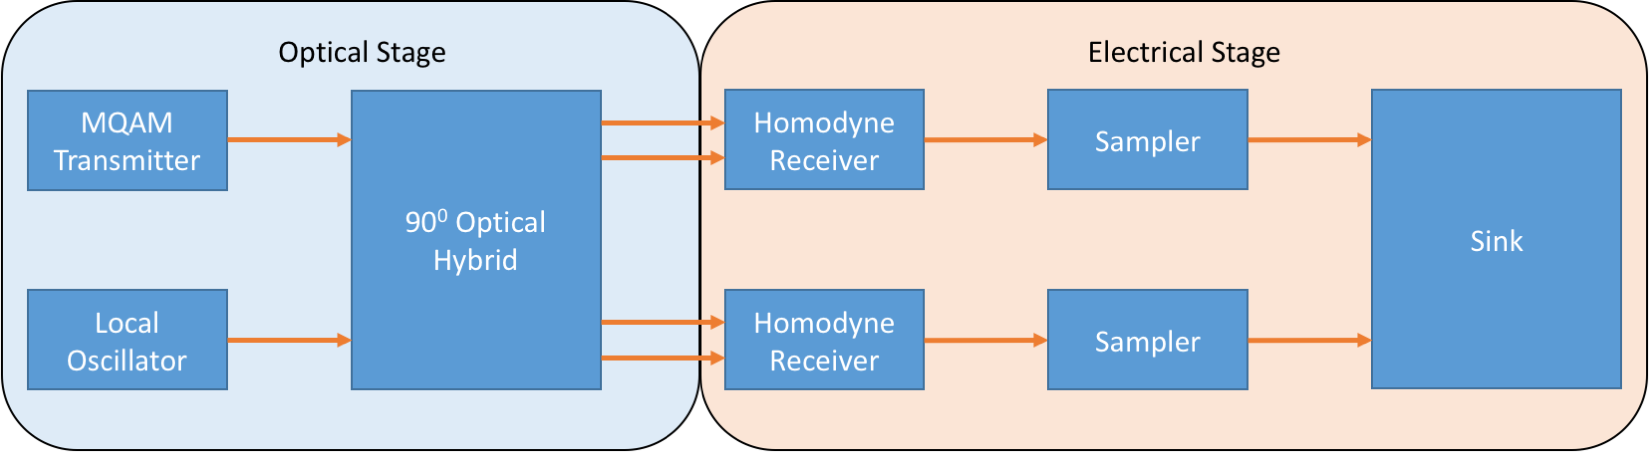
\includegraphics[width=\linewidth]{blockdiagramsimulation.png}
\end{center}
\end{frame}

\begin{frame}[t]{Simulation Parameters}
\begin{table}[H]
\centering
\begin{tabular}{|l|c|r|}
\hline
\textbf{Parameter}             & \textbf{Symbol} & \textbf{Value} \\ \hline
Detector Bandwidth             & $B$             & 800~GHz        \\ \hline
Symbol Period                  & $T$             & 20~ps          \\ \hline
Optical Wavelength             & $\lambda$       & 1550~nm        \\ \hline
Detector Responsivity          & $\rho$          & 1~A/W          \\ \hline
Detector Gain                  & $g$             & $10^6$         \\ \hline
Signal Optical Power           & $P_\text{Si}$   & $\sim51.26$~nW \\ \hline
Local Oscillator Optical Power & $P_\text{Lo}$   & 1~mW           \\ \hline
Thermal Noise Spectral Density & $N_\text{Th}$   & 1.610~V$^2$    \\ \hline
\end{tabular}
\end{table}
\end{frame}

\begin{frame}[t]{Simulation constellation}
\begin{center}
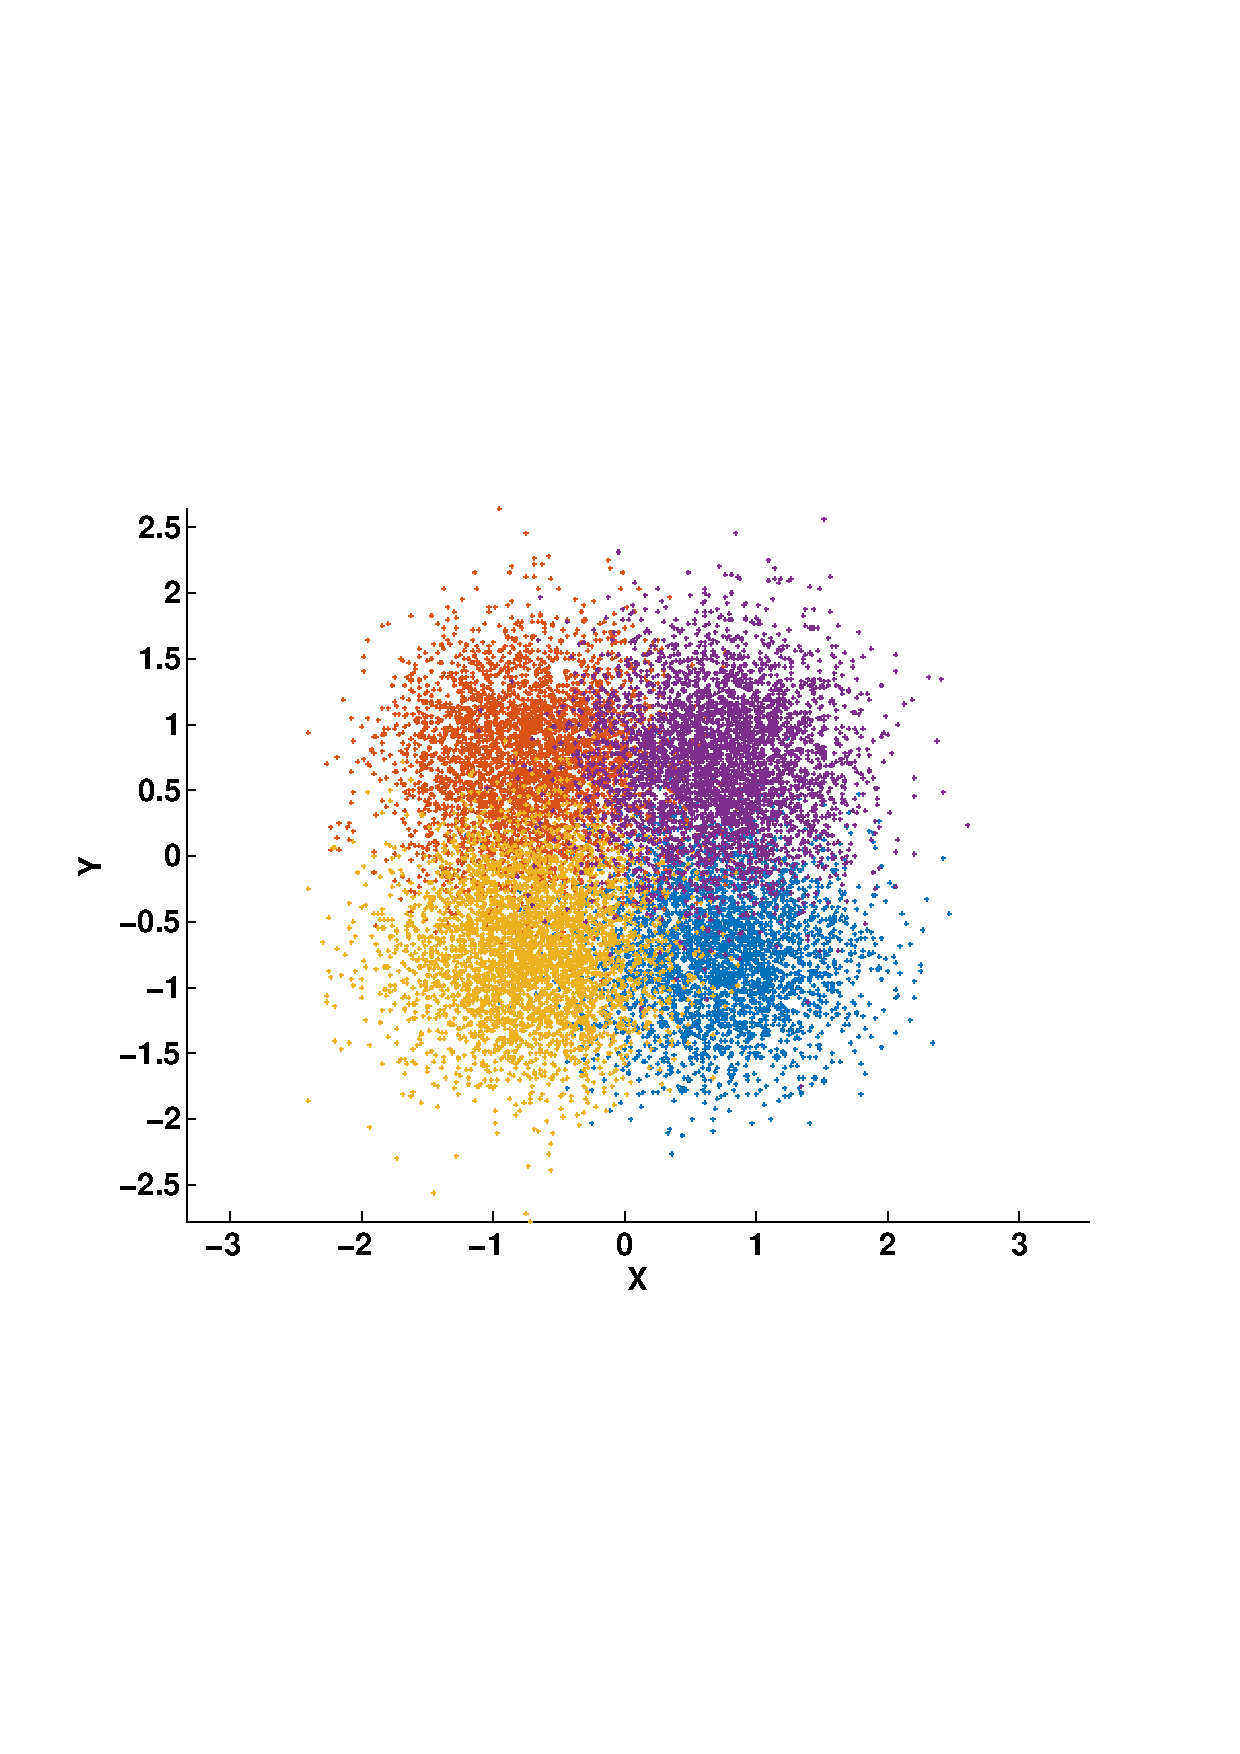
\includegraphics[width=.5\linewidth, trim={1cm 7cm 1.5cm 7.5cm}, clip=true]{constellationSimulation.pdf}
\end{center}
\end{frame}

\begin{frame}[t]{Noise characterization}
\begin{center}
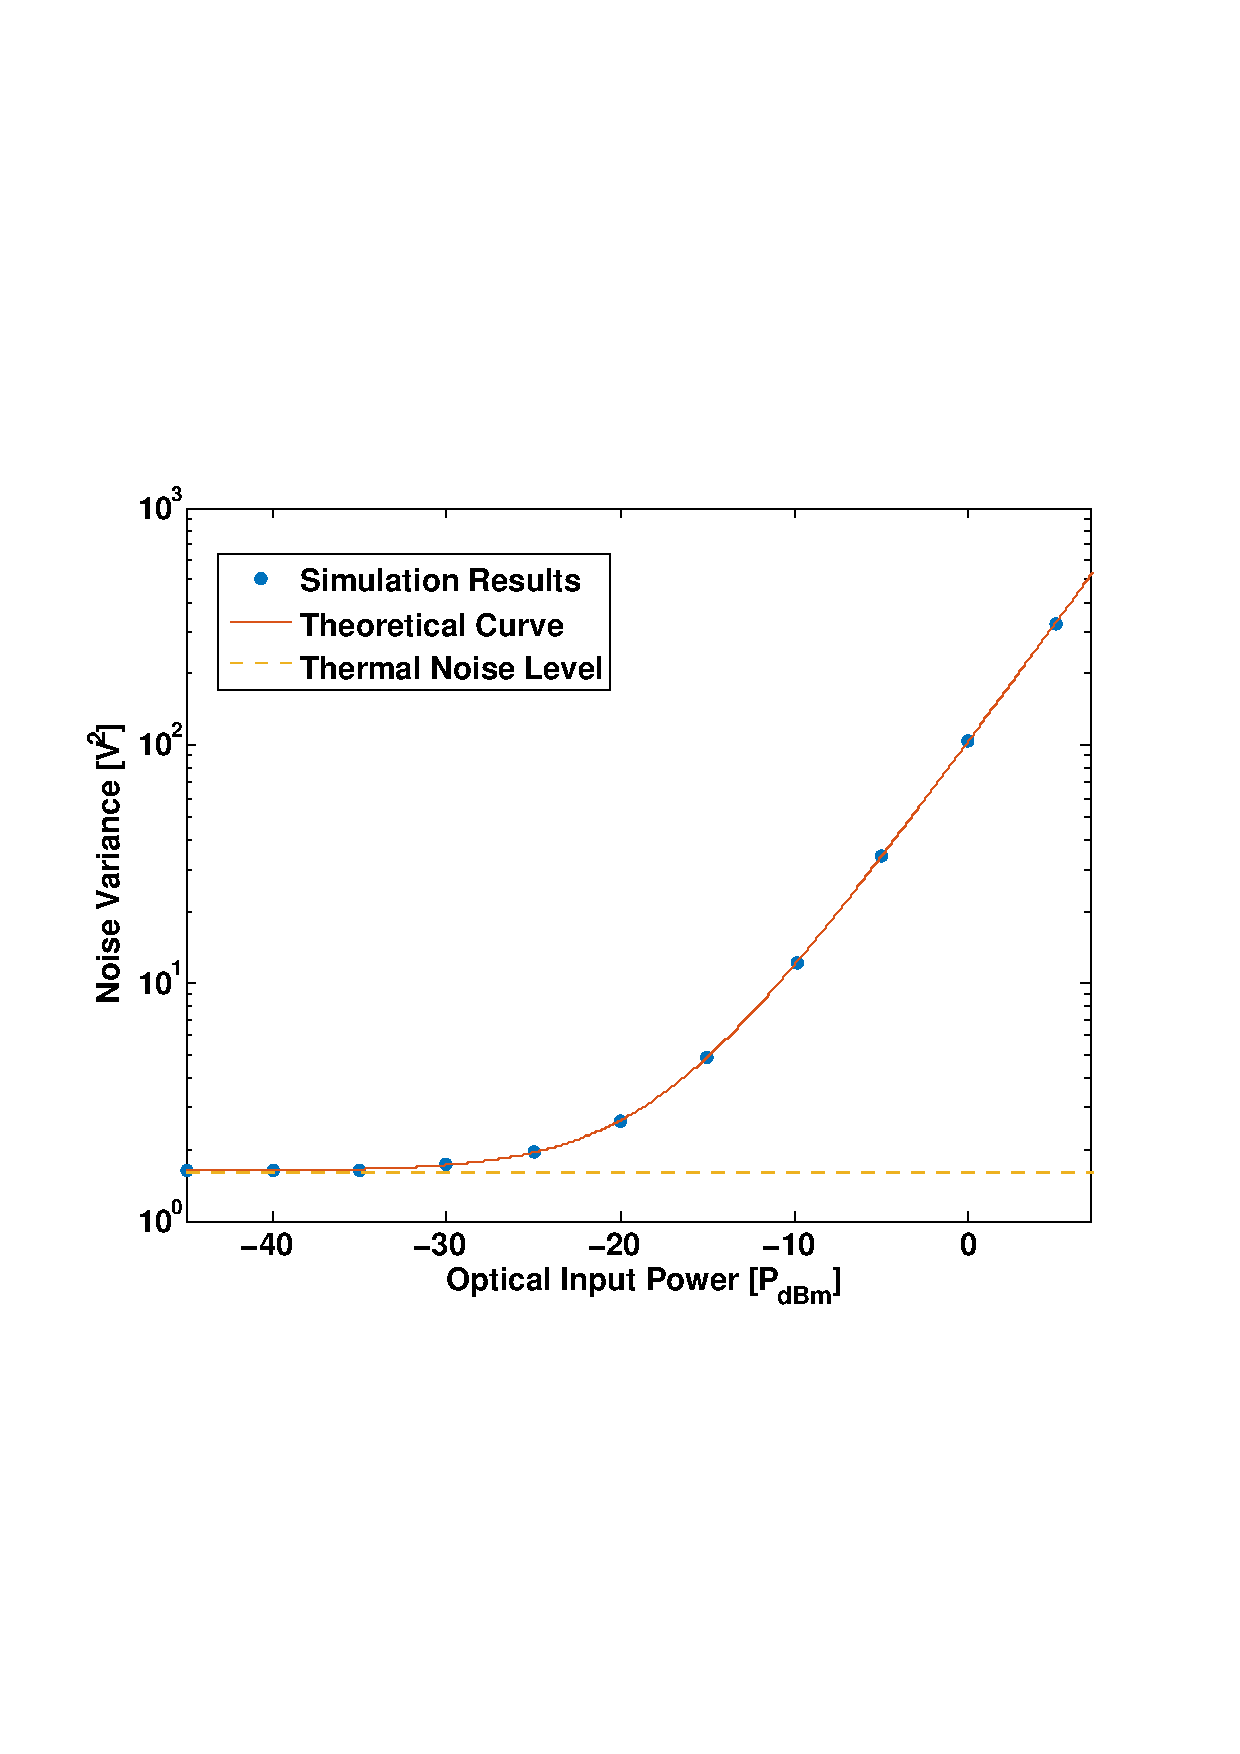
\includegraphics[width=.5\linewidth, trim={1cm 7cm 1.5cm 7.5cm}, clip=true]{simucharact.pdf}
\end{center}
\end{frame}

\begin{frame}[t]{Simulation secret key generation rate}
\begin{center}
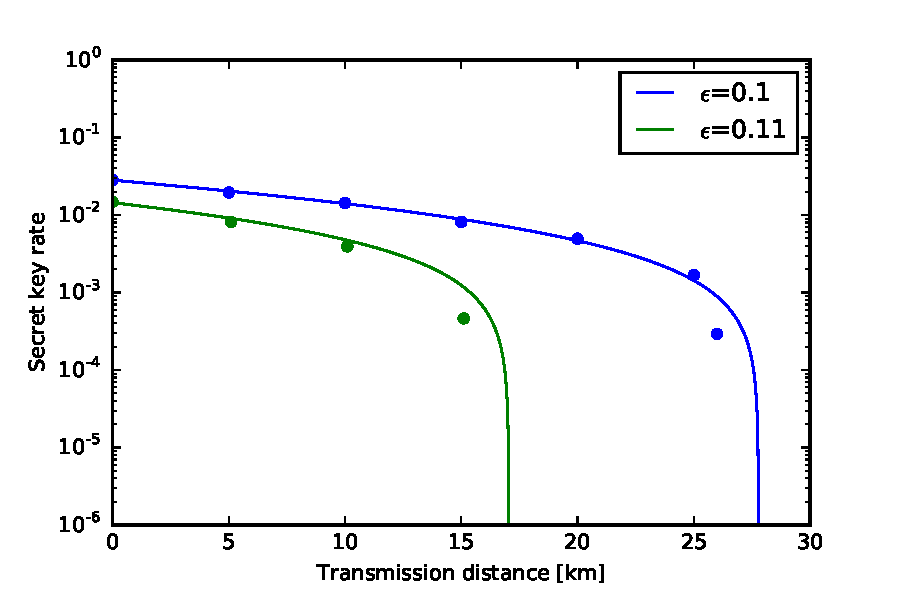
\includegraphics[width=.5\linewidth]{keyratesimulation.pdf}
\end{center}
\end{frame}

%%%%%%%%%%%%%%%%%%%%%%%%%%%%%%%%%%%%%%%%%%%%%%%%%%%%%%%%%%%%%%%%%%%%%%%%%%
%%%%%%%%%%%%%%%%%%%%%%%%%%%%%%%%%%%%%%%%%%%%%%%%%%%%%%%%%%%%%%%%%%%%%%%%%%
%%%%%%%%%%%%%%%%%%%%%%%%%%%%% section 4 %%%%%%%%%%%%%%%%%%%%%%%%%%%%%%%%%%
%%%%%%%%%%%%%%%%%%%%%%%%%%%%%%%%%%%%%%%%%%%%%%%%%%%%%%%%%%%%%%%%%%%%%%%%%%
%%%%%%%%%%%%%%%%%%%%%%%%%%%%%%%%%%%%%%%%%%%%%%%%%%%%%%%%%%%%%%%%%%%%%%%%%%
\section{Experimental}
\begin{frame}[t]{Experimental setup}
\begin{center}
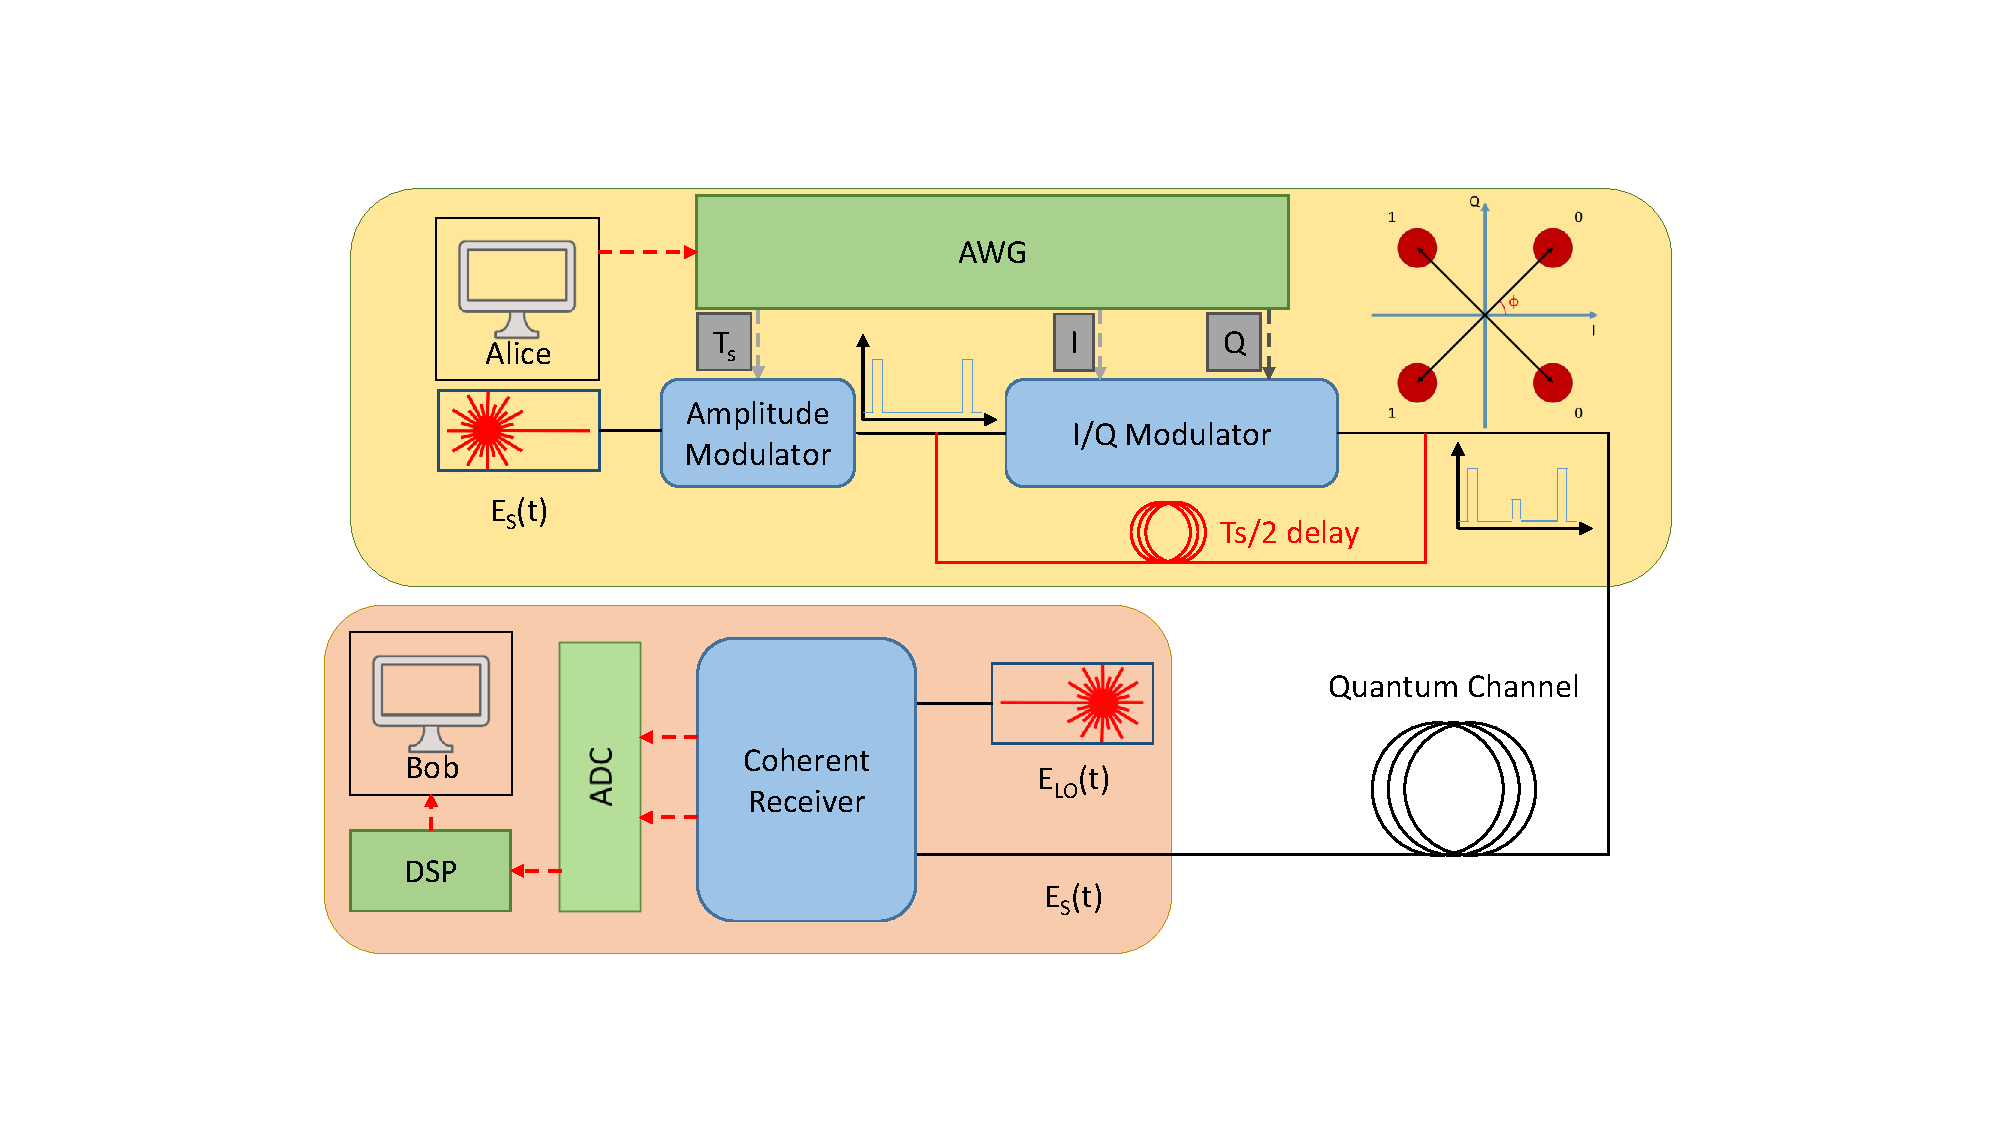
\includegraphics[width=\linewidth, trim={0cm 2.5cm 0cm 3cm}, clip=true]{withtrace.pdf}
\end{center}
\begin{itemize}
\item Laser wavelength, repetition rate, etc.
\end{itemize}
\end{frame}

\begin{frame}[t]{Phase drift compensation}
\begin{center}
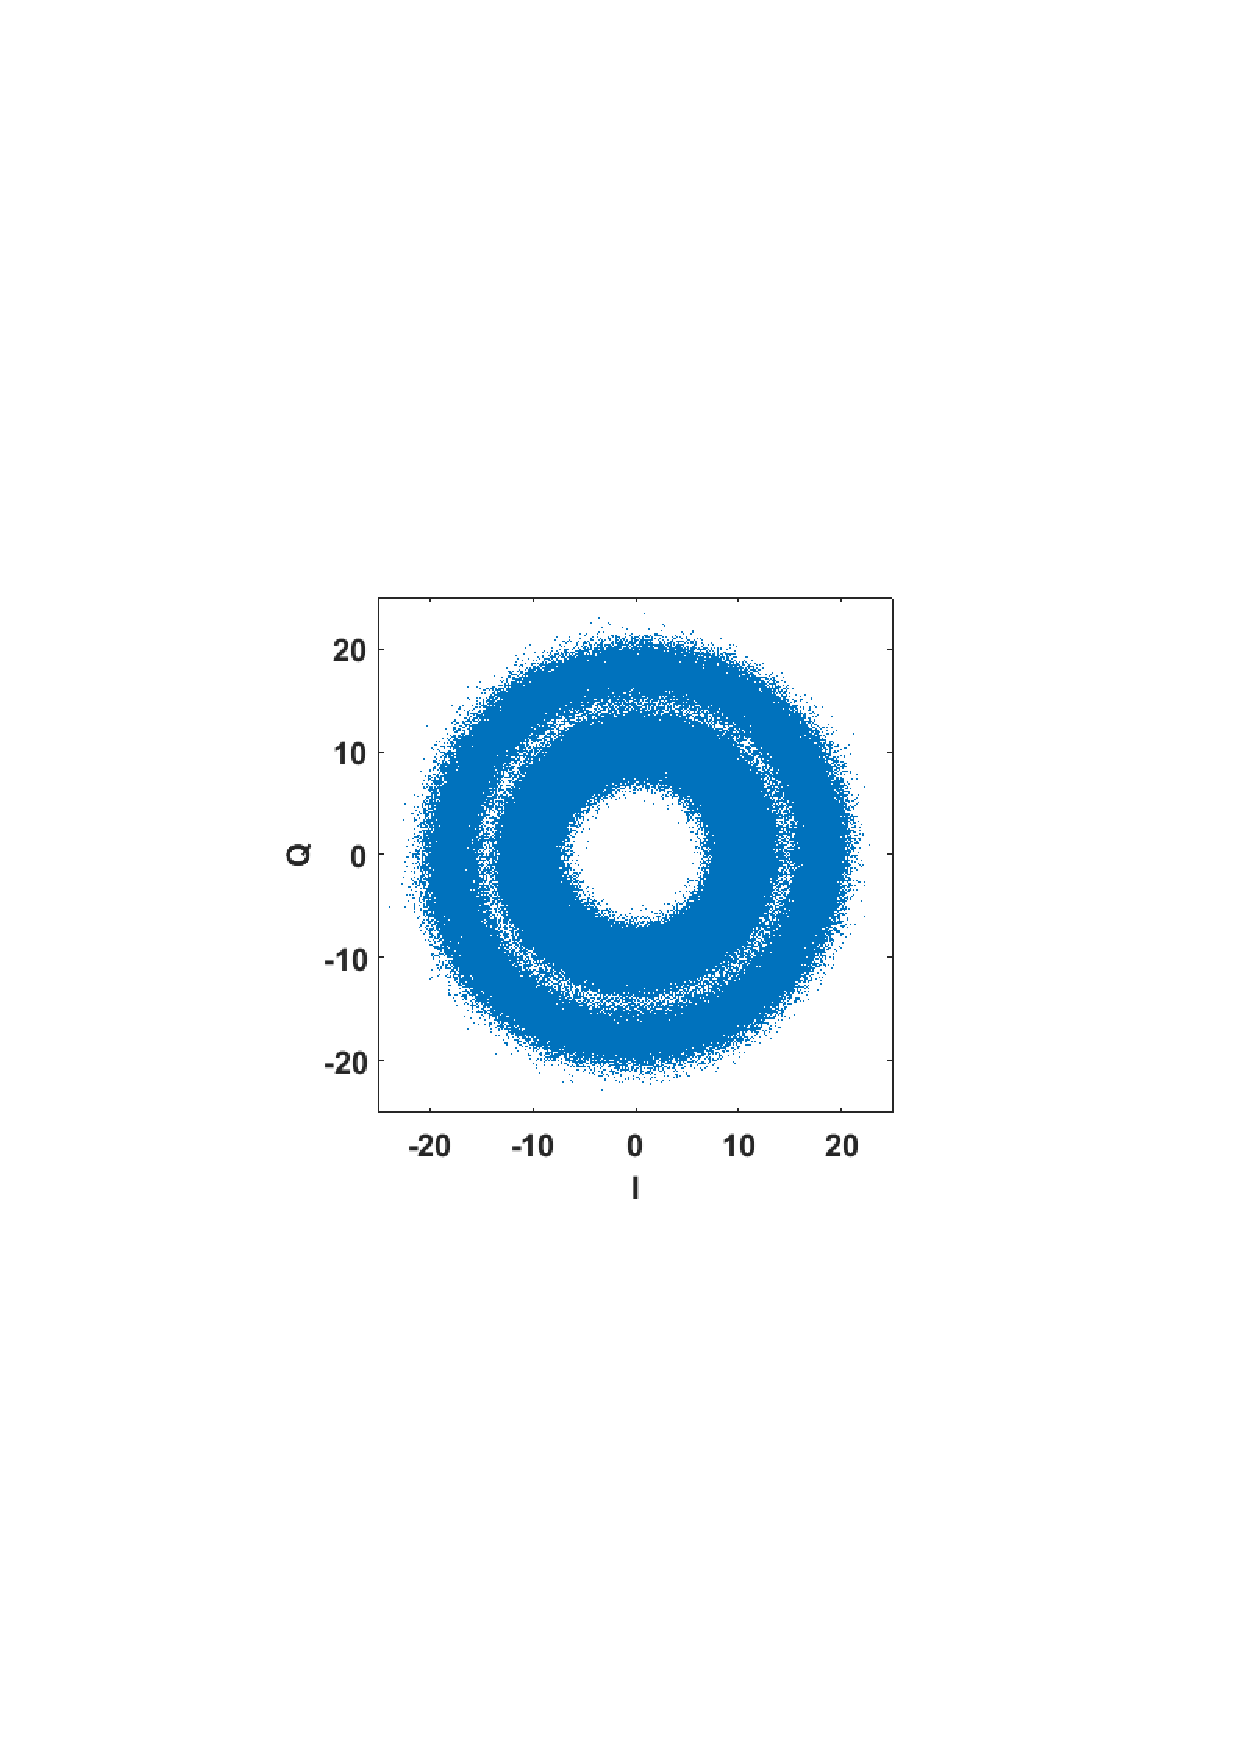
\includegraphics[width=.45\linewidth, trim={3cm 9cm 3cm 9.5cm}, clip=true]{beforephasedriftcompensation.pdf}
~
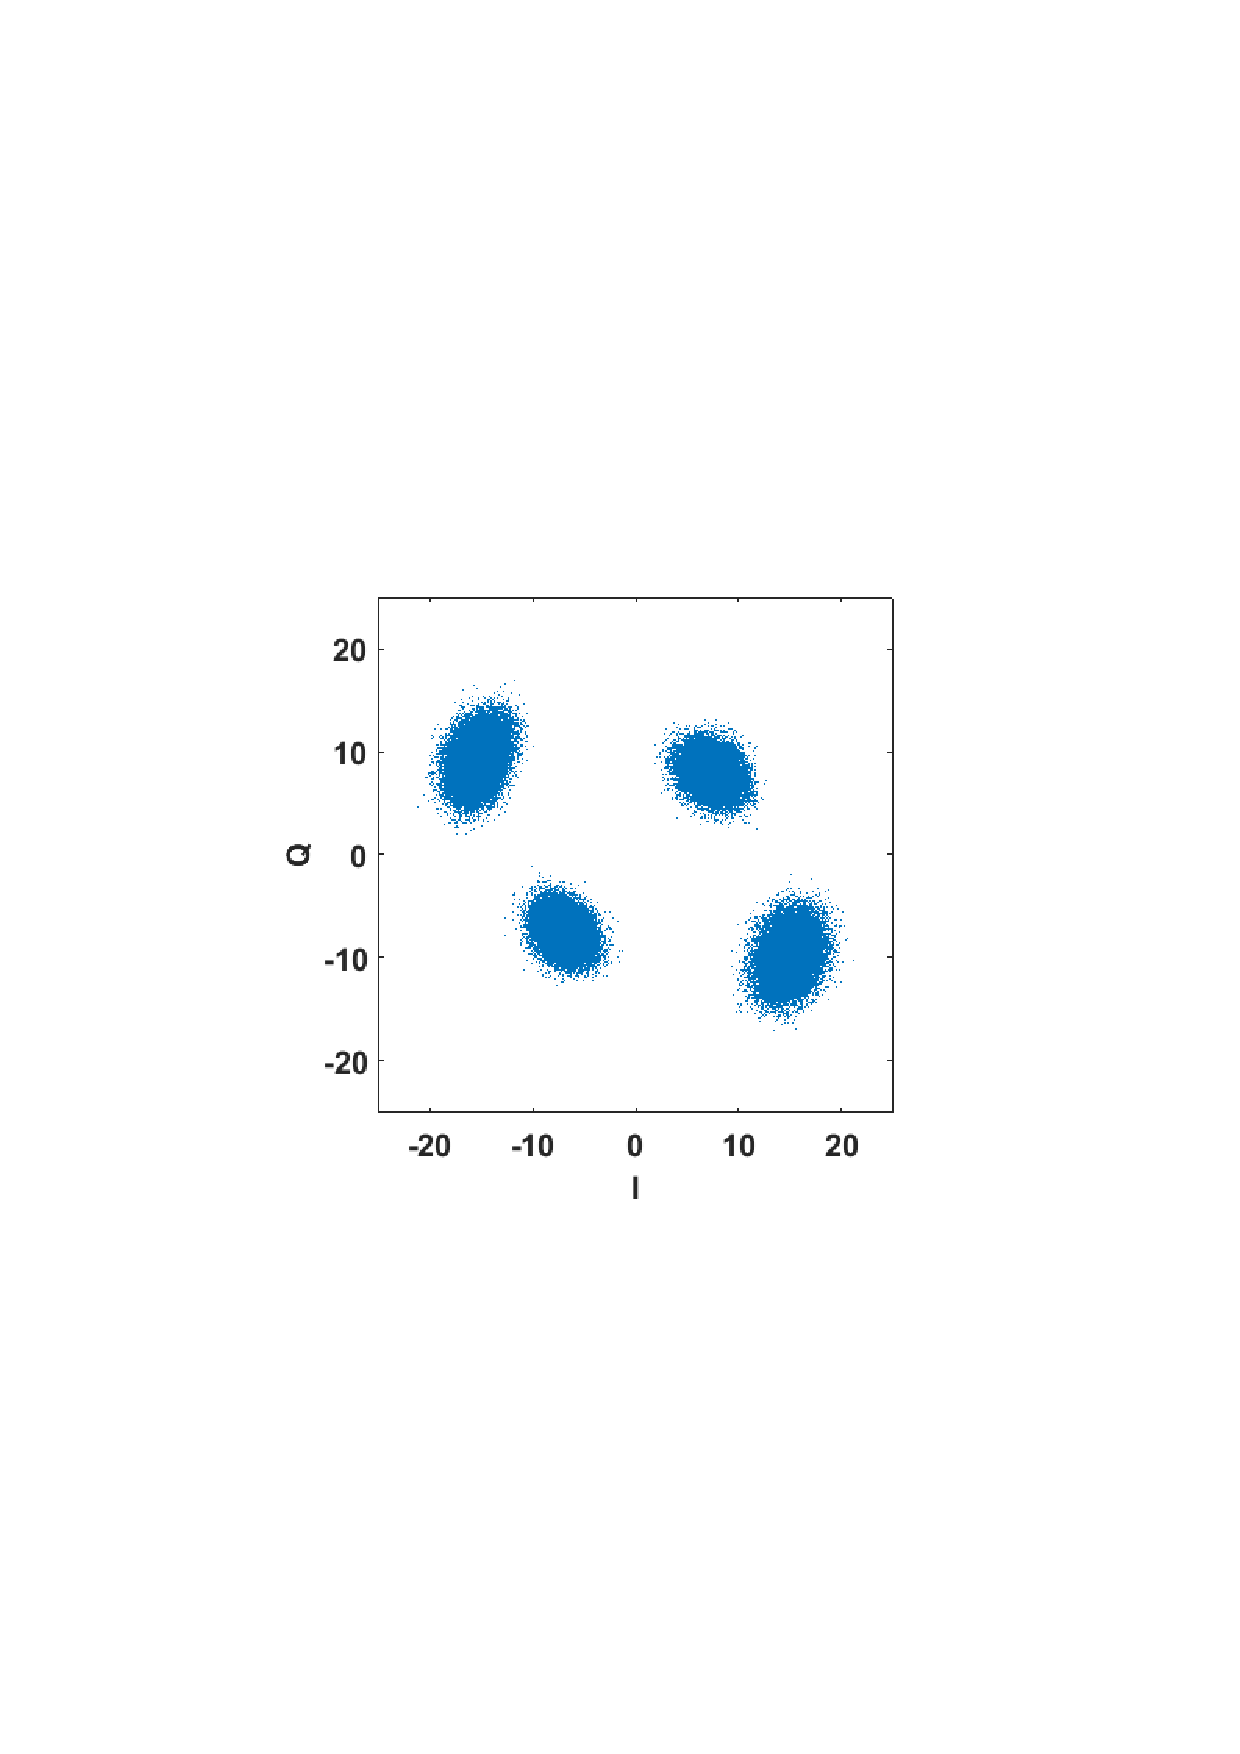
\includegraphics[width=.45\linewidth, trim={3cm 9cm 3cm 9.5cm}, clip=true]{afterphasedriftcompensation.pdf}
\end{center}
\end{frame}

\begin{frame}[t]{Detector noise variance characterization}
\begin{center}
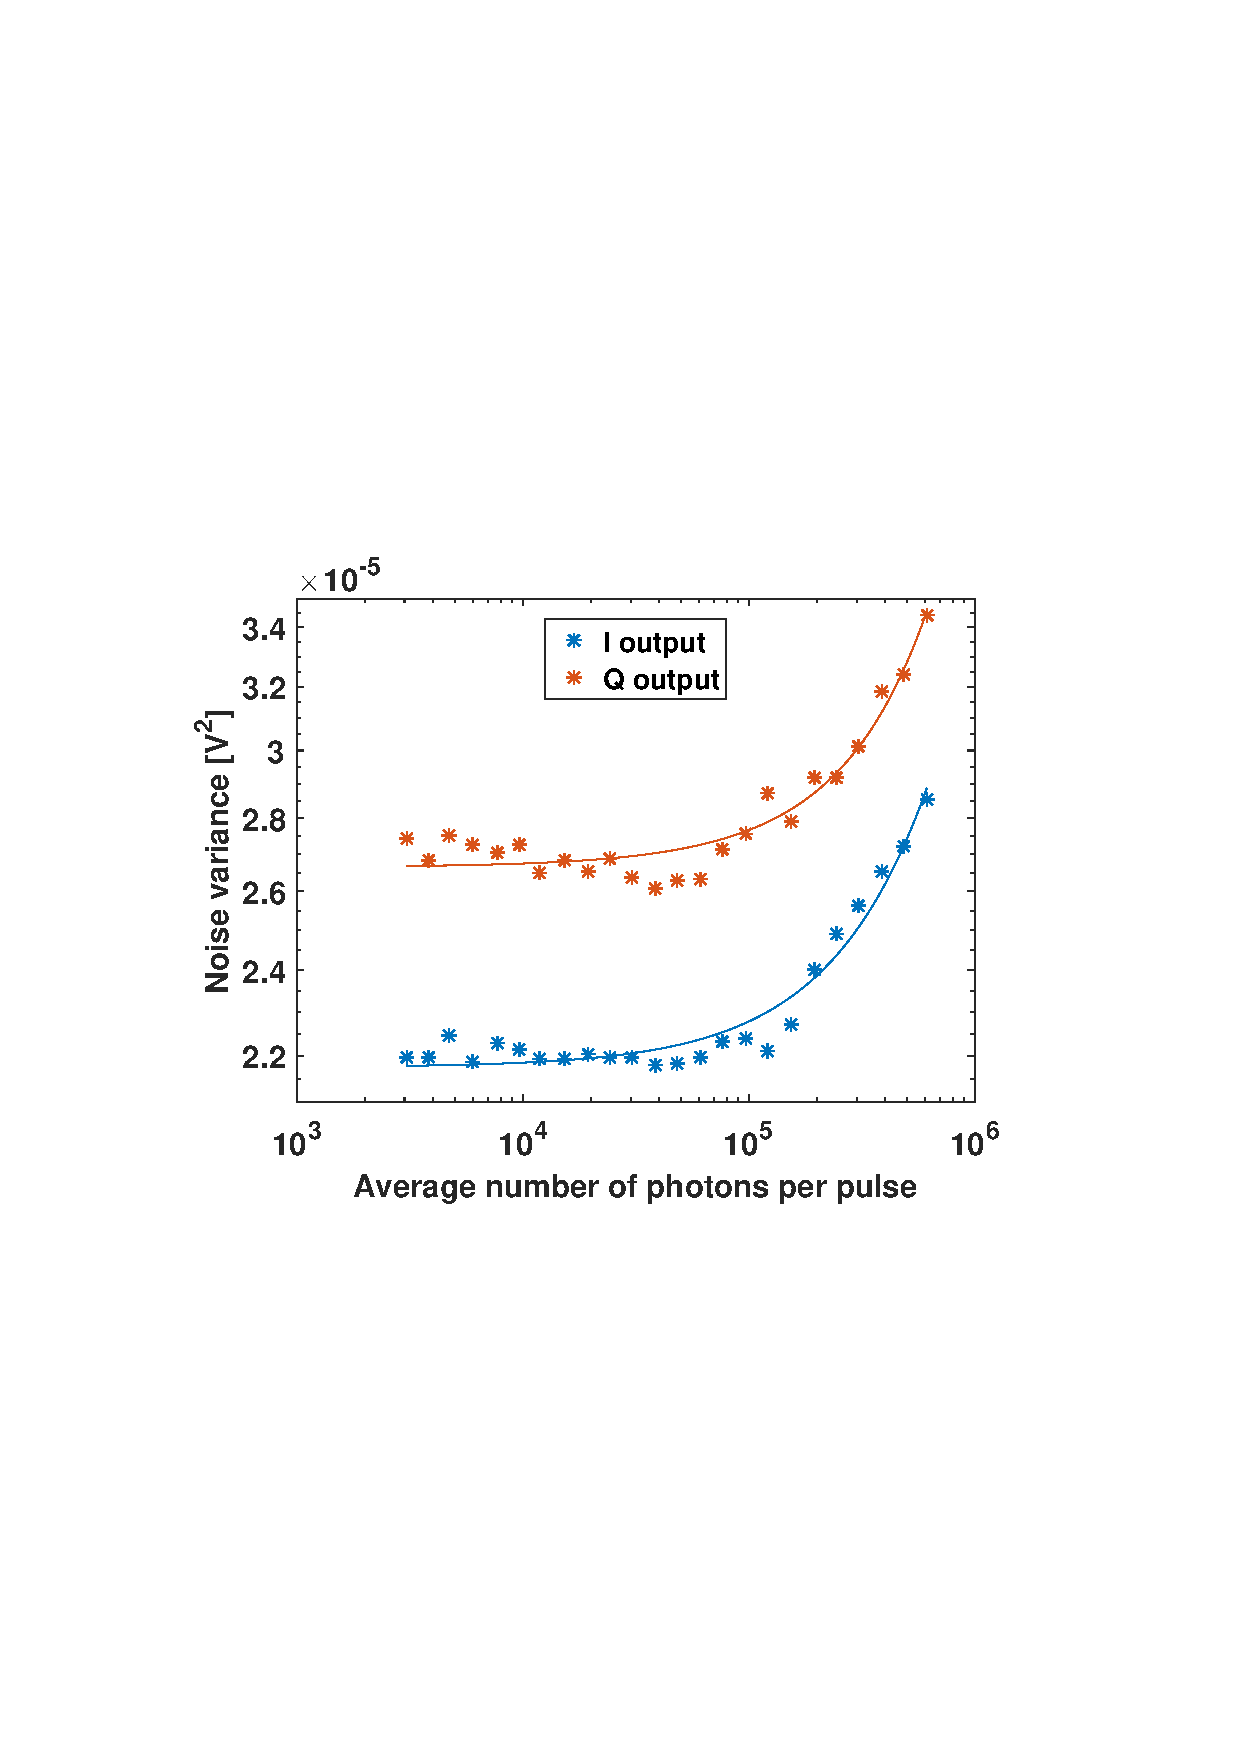
\includegraphics[width=.5\linewidth, trim={3cm 9cm 3cm 9.4cm}, clip=true]{characterizationInputLO.pdf}
\end{center}
\end{frame}

\begin{frame}[t]{Detector noise variance characterization}
The values of these coefficients in the two presented fits are:
$$a_0=2.18\times10^{-5}~\text{V}^2,$$
$$a_1=1.01\times10^{-11}~\text{V}^2,$$
$$a_2=2.481\times10^{-18}~\text{V}^2,$$
for the I output of the coherent receiver and:
$$a_0=2.67\times10^{-5}~\text{V}^2,$$
$$a_1=9.68\times10^{-12}~\text{V}^2,$$
$$a_2=5.22\times10^{-18}~\text{V}^2,$$
\end{frame}




%%%%%%%%%%%%%%%%%%%%%%%%%%%%%%%%%%%%%%%%%%%%%%%%%%%%%%%%%%%%%%%%%%%%%%%%%%
%%%%%%%%%%%%%%%%%%%%%%%%%%%%%%%%%%%%%%%%%%%%%%%%%%%%%%%%%%%%%%%%%%%%%%%%%%
%%%%%%%%%%%%%%%%%%%%%%%%%%%%% section 5 %%%%%%%%%%%%%%%%%%%%%%%%%%%%%%%%%%
%%%%%%%%%%%%%%%%%%%%%%%%%%%%%%%%%%%%%%%%%%%%%%%%%%%%%%%%%%%%%%%%%%%%%%%%%%
%%%%%%%%%%%%%%%%%%%%%%%%%%%%%%%%%%%%%%%%%%%%%%%%%%%%%%%%%%%%%%%%%%%%%%%%%%
\section{Conclusion}
\begin{frame}[t]
\begin{itemize}
\item 
\end{itemize}
\end{frame}

\end{document}